\section{Abbildungen: $\mathbb{R} \rightarrow \mathbb{R}^n$}

\subsection{Linearisierung}
$f(t+\Delta t) \approx f(t) + \Delta t \cdot f'(t)$

\subsubsection{Bogenlänge}
\begin{itemize}
	\item Normale Funktionen: $L_{a,b} \approx \int_a^b \sqrt{1+f'(x)^2} dx$
	\item Parametrisiert: \\
	\begin{displaymath}
		f: x \rightarrow
		\begin{pmatrix}
			f_1(x) \\ f_2(x) \\ f_3(x)
		\end{pmatrix}
		\Rightarrow
		L_{a,b} = \int_a^b \bigg |
		\begin{pmatrix}
			f_1'(x) \\ f_2'(x) \\ f_3'(x)
		\end{pmatrix}
		\bigg |_2 dx
	\end{displaymath}
	\item Bogenlänge Schraubenlinie:
	$L_{a,b} = \int_a^b (\sqrt{R^2 + v^2}\cdot \alpha ) d\alpha$
	\item Bogenlänge Zykloide:
	$L_{a,b} = \int_a^b (2 R\cdot sin(\frac{\varphi}{2})) d\varphi$
\end{itemize}

\subsubsection{Krümmung}
\begin{itemize}
	\item Normale Funktionen: $K(x) = \frac{f''(x)}{\sqrt{1+f'(x)^2}^3}$
	\item Parametrisiert: 
	$K(t) = \frac
		{\ddot{y} \dot{x} - \dot{y} \ddot{x}}
		{\big ( \dot{x} \sqrt{1 + \frac{ \dot{y} }{ \dot{x} }^2} \big )^3}
	$
	\item Krümmungskreis Radius: $\frac{1}{K(x)}$ \\
	\begin{figure}[h!]
		\centering
		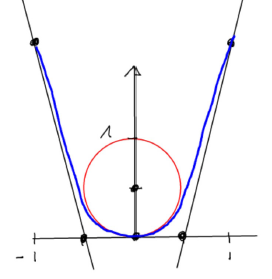
\includegraphics[scale=.5]{pics/kruemmungskreis}
		\caption{Krümmunkskreis im Scheitelpunkt}
	\end{figure}
\end{itemize}

\subsubsection{Kurven in Polarkoordinaten}
\begin{itemize}
	\item Archimedische Spirale (Sektorflächeninhalt):
	$\int_{\varphi_1}^{\varphi_2} (\frac{1}{2}\cdot r(\varphi )^2) d\varphi$
	\item Linienintegral:
	//TODO
\end{itemize}
